\scanpage{113}
\figure{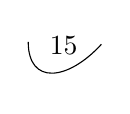
\begin{tikzpicture}[x=1cm,y=1cm]
\node at (0,0) {\mspage{15}};
\draw (-.45,.05) .. controls (-.45,-.5) and (.05,-.45) .. (.48,.02);
\end{tikzpicture}}

\diagram{\begin{tikzcd}[ampersand replacement=\&,row sep=small]
l_0^{-1}l_1l_0=\lambda_0\arrow[r,maps to]\&1\\
l_0^2=\lambda_{1/2}\arrow[r]\&l_0\\
l_1=\lambda_1\arrow[r,no head]\&l_1\\
l_\infty^2=\lambda_\infty\arrow[r,no head]\&l_\infty
\end{tikzcd}
\qquad
\begin{tikzcd}[ampersand replacement=\&,row sep=small]
l_0\arrow[r,maps to,no head]\&\varepsilon_0\\
l_1\arrow[r,maps to,no head]\&l_1\\
l_\infty\arrow[r,no head]\&\varepsilon_\infty
\end{tikzcd}}

\[
\varepsilon_\infty l_1\varepsilon_0=1
\qquad\text{i.e.}\qquad
\underbrace{\rho^{-1}\sigma_\infty\deleted{\rho^{-1}}}
\underbrace{\deleted{\rho}\deleted{\sigma_\infty}
\deleted{\rho}\deleted{\sigma_\infty}}
\deleted{\sigma_\infty}\deleted{\rho}
=\rho^{-1}\sigma_\infty
\]

\[
\begin{aligned}
\varepsilon_0&=\sigma_\infty\rho\\
\unsure{\varepsilon_1|l_1}&=\rho\sigma_\infty\\
\varepsilon_\infty&=\rho^{-1}\sigma_\infty\rho^{-1}
\end{aligned}
\]

\margin{112}
